\newpage
\section{零售管理系统}
\label{sec:foundation}

\subsection{服务器}

\begin{figure}[htbp]
	\centering
	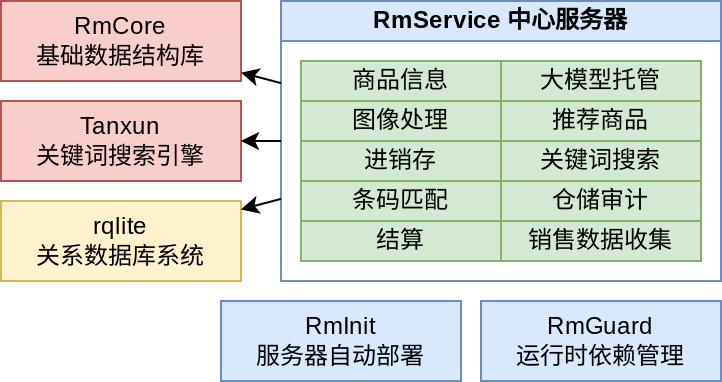
\includegraphics[width=0.8\textwidth]{./imgs/arch-server.png}
	\caption{本设计的服务器整体设计图示:其中蓝色表示相互独立的应用程序,绿色表示服务器的功能,红色表示功能库,黄色表示第三方库或应用程序,箭头表示被指方受到依赖。}
	\label{fig:arch-server}
\end{figure}

\subsubsection{数据结构}
如图 \ref{fig:arch-server} 所示,因为采用了客户端-服务器设计模式,该系统所有业务相关信息统一由RmService模块进行管理。因此,为了在系统中体现充分的可维护性、可拓展性,实际对数据进行存储的关系数据库系统rqlite原则上无法被客户端(各个商家端、顾客端应用程序)所直接访问,而是由RmCore所定义的数据结构进行封装。

\begin{figure}[htbp]
	\centering
	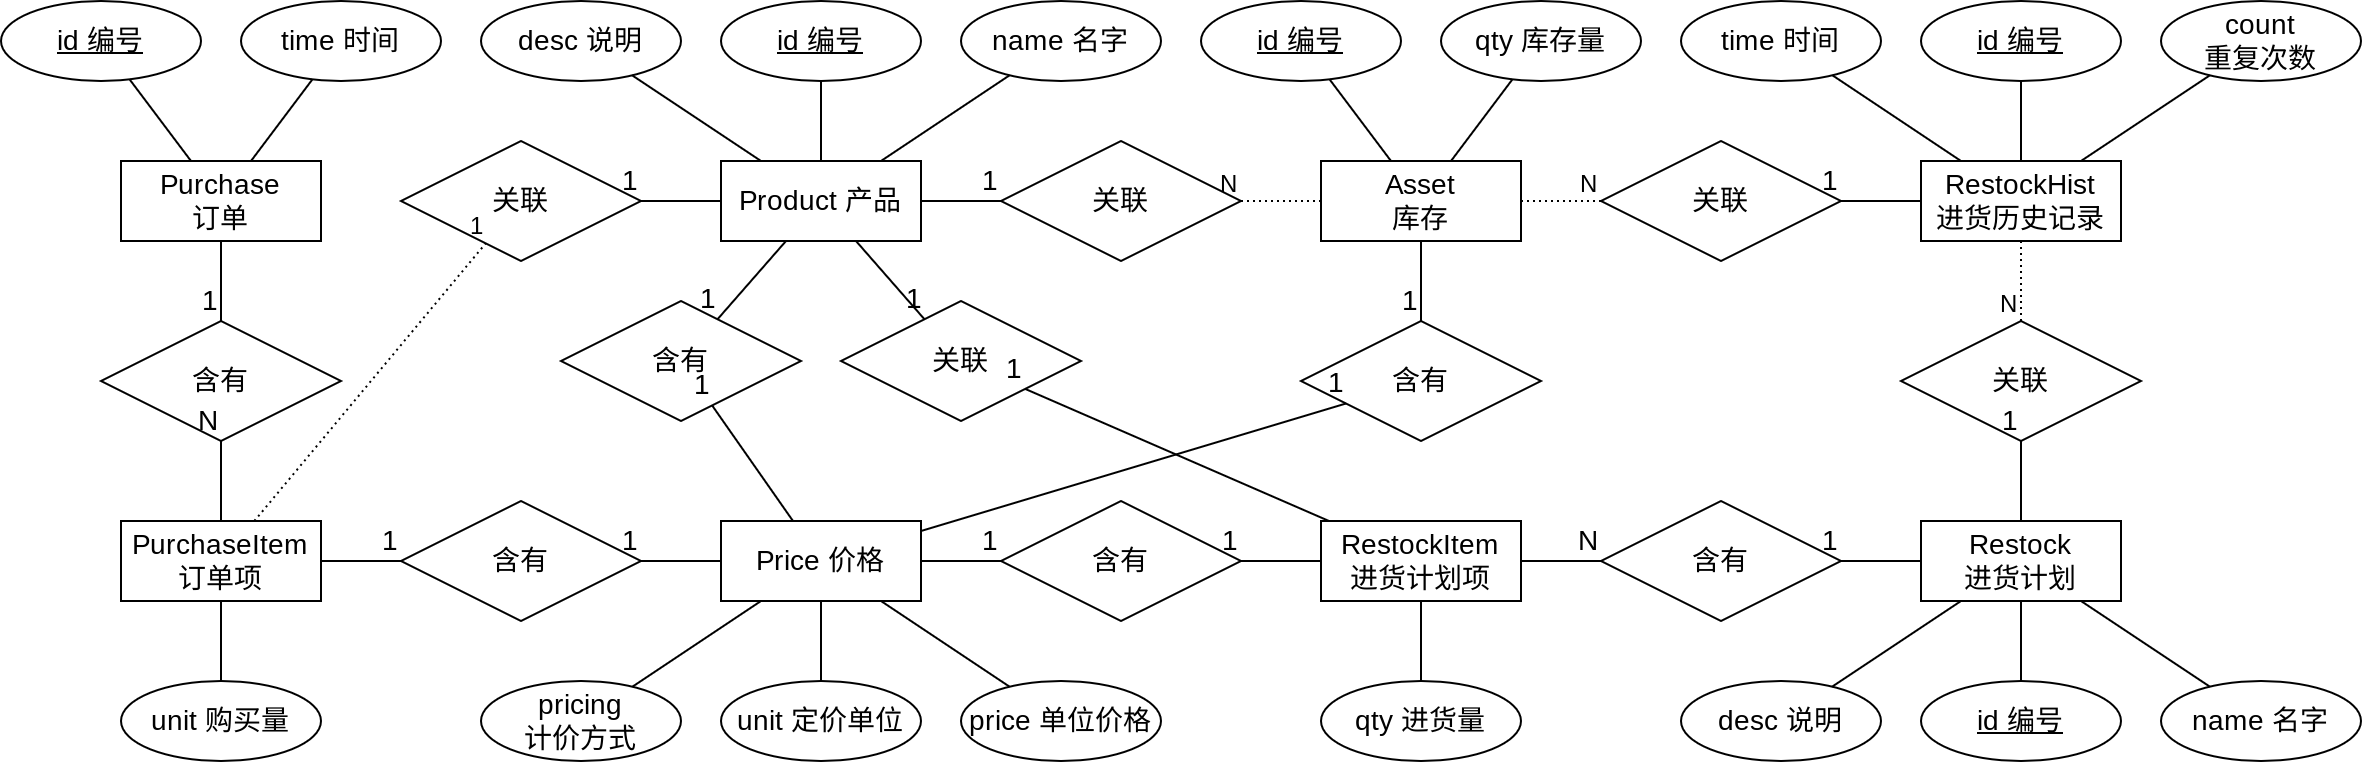
\includegraphics[width=0.8\textwidth]{./imgs/rms-er-rmcore.png}
	\caption{RmCore模块所定义数据结构的实体关系图}
	\label{fig:rms-er-rmcore}
\end{figure}

如图 \ref{fig:rms-er-rmcore} 所示,该模块定义了在零售经营过程中会利用到的各种(需要持久化存储的)数据结构,并且已经以面向对象的、有利于代码复用、序列化和反序列化和有利于在不同开发环境下形成统一接口的方式进行封装。为了便于在数据库中以整数方式存储许多常常为小数的数据,规定任何直接代表金钱数量的值以人民币分为单位,任何直接代表物体质量的值以克为单位。

其中值得注意的一个类型是库存“Asset”。为了便于对库存所对应的进货批次、进货价格等信息进行跟踪,每一个库存项都与一个进货历史记录项目“RestockHist”相关联。因此,同一个产品可以因为多次不同进货并且较老进货批次剩余产品尚未被消化完毕而存在多个库存条目。同样地,只需要统计一个RestockHist所对应的Asset,便可以统计某一个批次进货的消化情况。

另一个较为特殊的类型是价格“Price”。考虑到不同零售商品类型定价策略的区别,该类型的属性计价方式“pricing”为具有“Package”(按件)和“Weight”(按重量)两个可能值的枚举。而属性定价单位“unit”在按件计价时代表属性价格“price”对应的商品件数,反之则是克数。而将属性price和unit分离(而不是表示为单位价格)有助于避免如“十元三件”(一件$\frac{10}{3}$元)此类出现整数或IEEE 754浮点类型数字无法准确表示的数值的情况。

\begin{figure}[htbp]
	\centering
	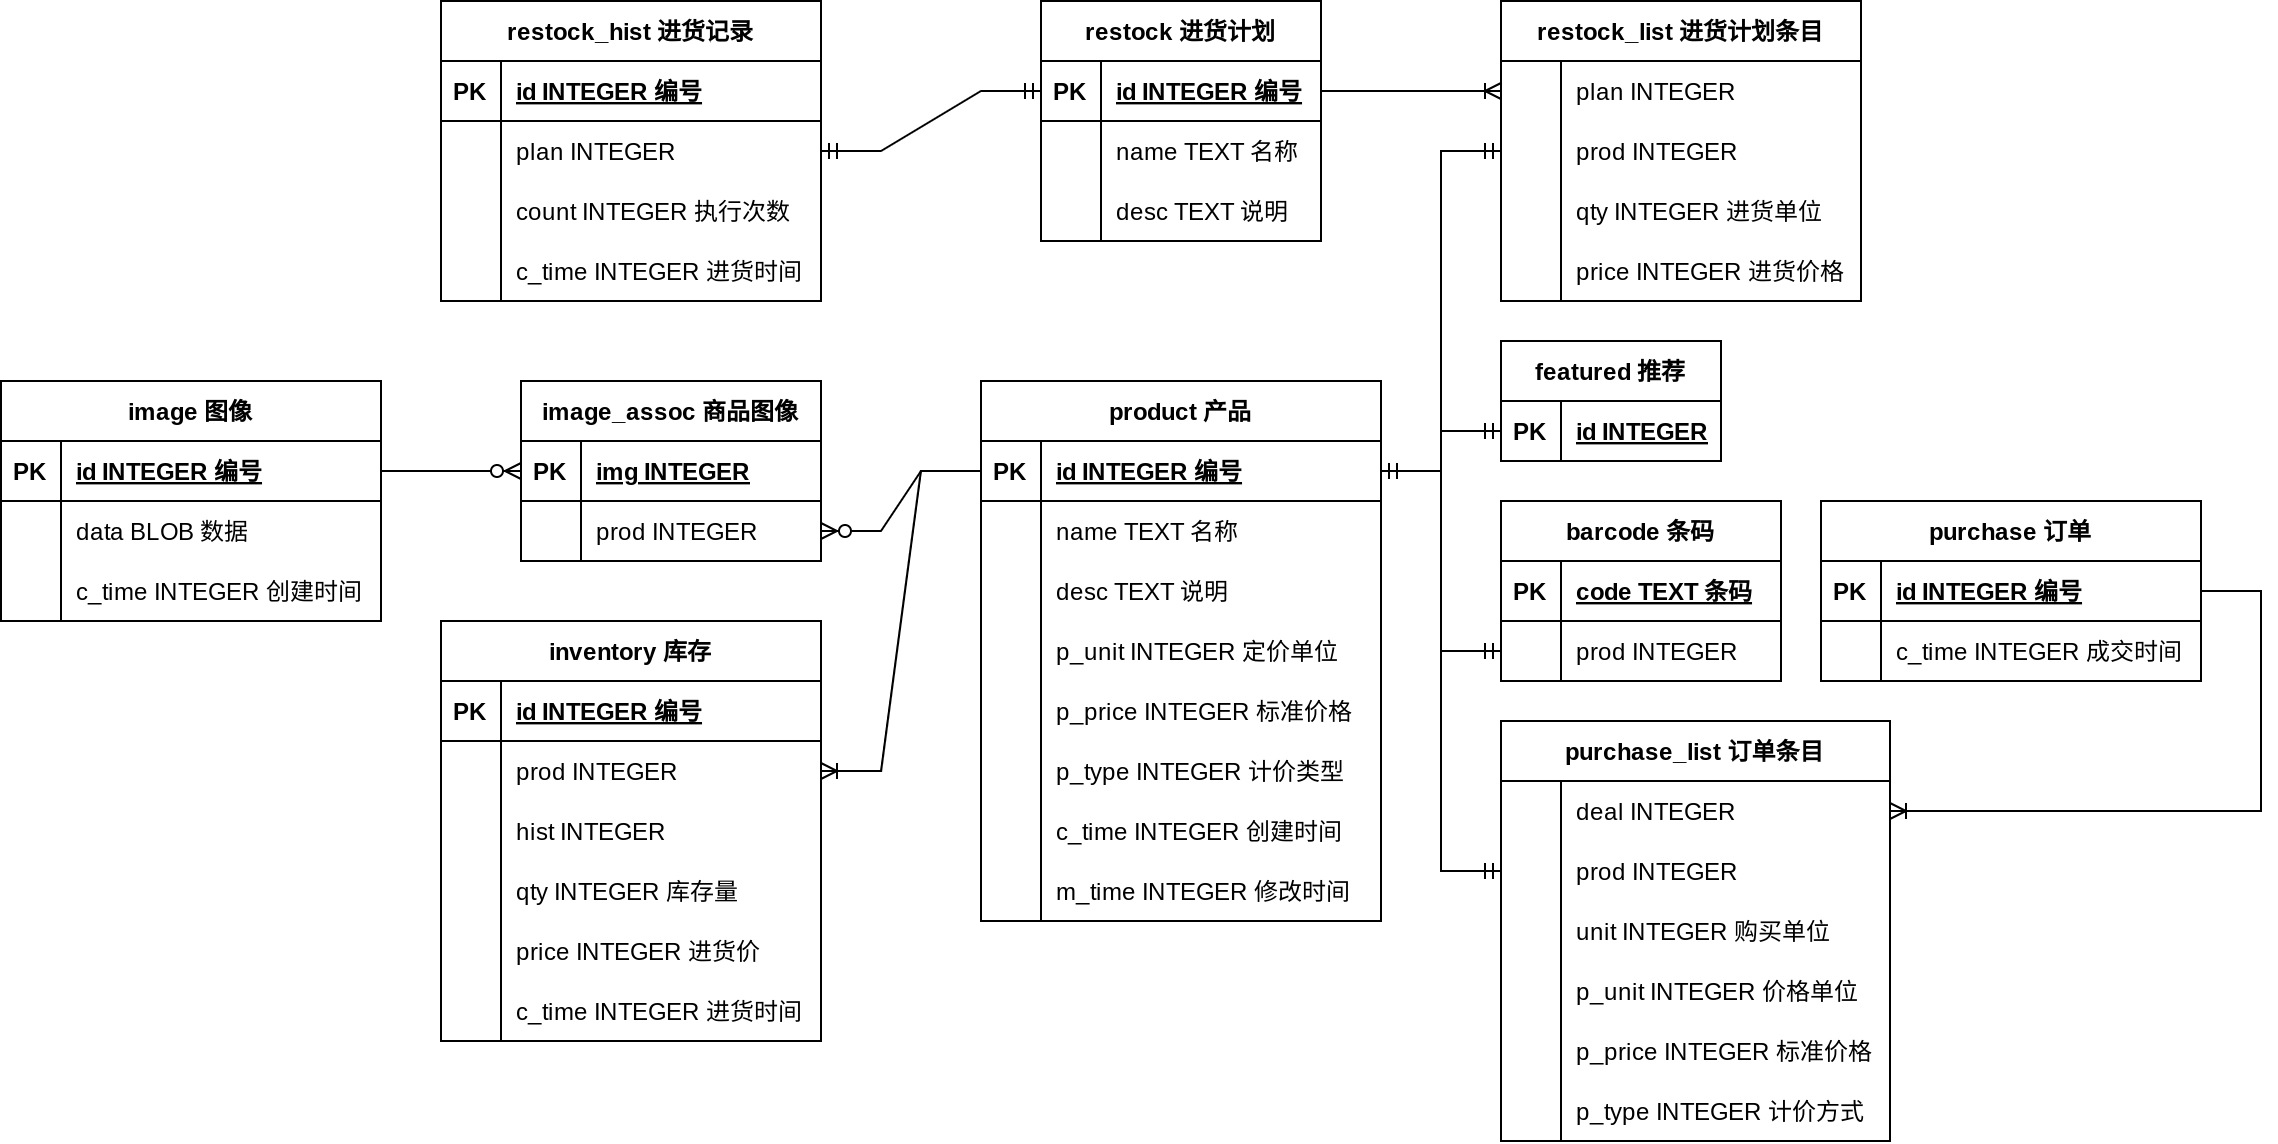
\includegraphics[width=0.8\textwidth]{./imgs/rms-db.png}
	\caption{数据库中存储数据格式的实体关系图}
	\label{fig:rms-db}
\end{figure}

图 \ref{fig:rms-db} 所描绘的是 \ref{fig:rms-er-rmcore} 所示的模型还有少数以其他方式封装的数据的在关系数据库系统中的实际存储方式。除了Price类型没有单独表格,而是被扁平化地存储在了各个表中的区别,数据存储的方式基本与封装成一比一对应关系。少部分表格具有额外的创建、修改时间字段(“\verb|c_time|”和“\verb|m_time|”)留作未来拓展使用。值得注意的是,为了改善大规模访问的效率,商品图像数据并不是存储在外部文件系统,而是和其他资料一同存储在数据库中。

\subsubsection{应用程序接口}
为了实现各个客户端应用程序与服务器的有效信息交换,服务器采用HTTP协议进行信息传递,即服务器实现面向客户端应用程序的HTTP API。由于API覆盖范围较广、数量较大并且功能迥异,故该课题代码开发时大部分API端点设计遵从如下规范:

\begin{itemize}
	\item 期望请求主体(body)部分带有实际数据者,接受POST方法的请求;否则接受GET方法的请求,并且对方法错误的请求响应“Not Found”状态。
	\item 期望请求主体带有多于一个字段者,接受使用JSON格式序列化的数据,否则按实际情况决定主体数据类型。
	\item 较短、较少的请求参数,可以通过HTTP地址参数而不是请求主体传递。
	\item 除纯二进制数据(如图片)外,方法一律使用JSON格式序列化返回值。
	\item 在端点调用遇到责任在客户端(调用参数格式错误等)的问题时,返回“Bad Request”状态并且尽可能在回复主体中包含对问题根源进行描述的字符串。
	\item 同上,但责任在服务器(意外情况)时,返回“Internal Server Error”状态并且在主体中包括导致问题的函数调用返回的相关错误信息。
	\item 客户端请求的资源或任务结果尚未准备完成时,返回“Accepted”状态并在回复主体中标注具体任务现状。
\end{itemize}

为了支持商家端应用程序中对某些数据条目的高级搜索功能,服务器对某些数据类型提供了封装程度较低的请求方式,即允许部分客户端应用程序自行合成并向服务器提供用于数据获取的SQL查询 \verb|SELECT| 调用参数中的 \verb|WHERE| 子句。值得注意的是,该特性因为受到的自动检查、合法性担保较少而具有一定的危险性,不合理的使用可以引发较严重的安全隐患。因此,只有特定商家端的功能将会使用到这个API终点,并且子句的合成也会(在客户端)受到一定的规范和限制。

\subsubsection{自动部署}
不难发现,该设计所实现功能板块领域跨度较大,在原理、技术路线和使用环境要求上不尽相同,甚至在某些情况下相差甚远,所以部署的难度和复杂程度是比较高的。因此,该设计包含一个利用与服务器相似的技术路线开发的自动服务器部署应用程序RmInit。

该程序具备利用系统命令执行和命令输出检测该设计中各个功能模块在该程序所运行的设备上运行所依赖的第三方软件库或执行环境是否正确安装的功能;具备使用系统自带下载工具(如 \verb|wget| )自动从互联网上下载对应该程序所运行的设备的体系结构的rqlite应用程序合集,并且在部署的系统上运行数据库初始化脚本的功能;能够按照预先准备的应用程序项目列表逐个运行对应的编译任务并复制编译输出的二进制程序,支持使用 \verb|uv| 托管的Python项目、使用Gradle项目管理工具的Java-Kotlin项目、基于CMake项目管理工具的C++项目和使用Cargo命令管理的Rust可执行程序项目目标。

为了适应在多设备分布式系统中正确分配各设备功能特性、规避在特定平台无法完成编译任务的应用程序,RmInit采用了 \verb|clap| 命令行参数分析器,支持利用命令行参数控制大部分功能的包含与否、部分配置文件的覆盖与否。

此外,该应用程序还实现了可选的配置文件升级功能。配置文件升级是一个递归的过程,每一次调用都由新配置和旧配置(或者它们的一部分)参与。若新旧配置均为基本值类型且类型一致,则旧配置受到保留。若新旧配置类型、结构不一致,则使用新配置取代之。若新旧配置为键值表,则利用旧表内容覆盖新表,每个元素的覆盖递归执行该过程。

\subsubsection{服务依赖管理}
服务器中不同应用程序可能存在一定依赖关系,比如RmService依赖于rqlite关系数据库管理系统,此时合理安排各个应用程序或后台服务的启动顺序对系统整体稳定程度将会有所帮助。因此,服务器工具软件中包含RmGuard服务器运行时依赖管理,支持按网络请求启动或停止相关服务的服务器守护程序。该应用程序内置服务器中不同模块二进制程序之间的依赖关系,并且启动时将会读取对应的配置文件。不论使用任何方式(自启动或按需启动)来唤起任何模块,都会触发对应程序所依赖的模块(若尚未启动)的启动过程。

\subsubsection{图像存储}
为了顺利在较为受到限制的存储空间内存放潜在的海量商品图像,并且改善各应用程序获取商品图片的速度、降低网络带宽压力,服务器具备自动对图像进行缩放和压缩的功能。服务器所接受的图片(已编码的数据)首先会被解码,然后将被在保持图片原本宽高比的情况下,将图片较长一边的长度限制在300以内,并按需调整另一边,并利用较为快速的双线性插值办法进行重采样。程序将逐个尝试100、95、90\ldots60、55的JPEG压缩率对图片进行编码,直到使用了最大压缩率或图像大小小于配置文件制定阈值为止。

\subsection{管理界面}

\begin{figure}[htbp]
	\centering
	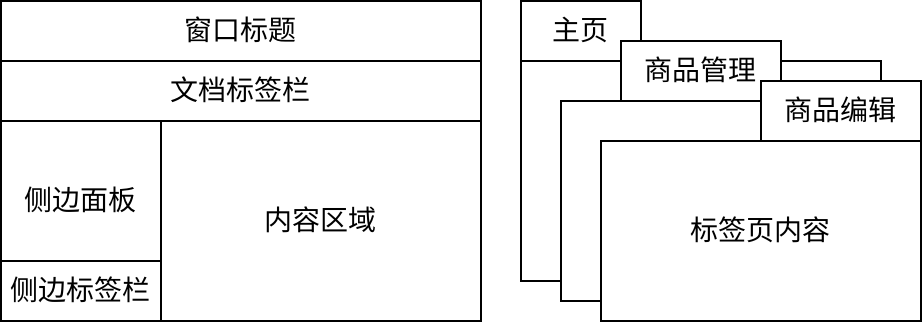
\includegraphics[width=0.8\textwidth]{./imgs/rma-design-layout.png}
	\caption{左侧:桌面商家端的用户界面布局;右侧:多个文档标签的实例}
	\label{fig:rma-design-layout}
\end{figure}

为了充分利用面向桌面型计算机开发的应用程序的操作效率高的特性,管理界面模块采用如图 \ref{fig:rma-design-layout} 所示的按标签页分文档的UI组织方式,其中大部分标签页采用主要内容板块加侧边栏展示额外信息的布局方式,以增强对键盘鼠标操作的友好性。鉴于许多种类的零售业务资料可以被抽象为同一种类型的多个不同实例,并且具有同样的对理解数据内容较为重要的字段(如名称、说明),故决定以表格方式对其进行整理。管理界面具备如下的功能:

\begin{itemize}
	\item 商品管理
	\begin{itemize}
		\item 创建或编辑商品
		\item 检索、查看和管理既有商品
	\end{itemize}
	\item 库存管理
	\begin{itemize}
		\item 管理、预览和执行进货计划
		\item 查看仓储情况
		\item 管理仓储审计批次
	\end{itemize}
	\item 编辑推荐商品
	\item 管理商品图片
\end{itemize}

\begin{figure}[htbp]
	\centering
	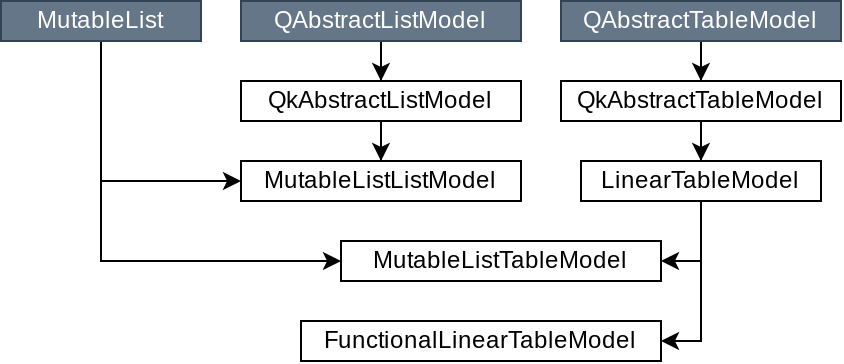
\includegraphics[width=0.8\textwidth]{./imgs/rma-tables.png}
	\caption{用于表格组件的模型类继承关系:灰色框代表第三方库或开发环境带有的类,箭头指向子类或者实现该接口的类。}
	\label{fig:rma-tables}
\end{figure}

不同表格模型(向表格组件提供数据的对象)类之间的继承关系如图 \ref{fig:rma-tables} 所示,其中 \verb|MutableListListModel| 和 \verb|MutableListTableModel| 在表格模型中整合了可变不定长数组的特性,可以将开发模型中的对象数组与对应对象集合在UI上的展示相同步,避免繁重的界面开发任务,以此简化数据映射的开发复杂程度。

此外,管理界面的许多作为既有信息展示方法的表格组件还具备通过键盘快捷键或右键菜单进行搜索结果整理、复制或粘贴的功能,从业者可以通过在不同的搜索结果、功能模块之间粘贴剪贴板中编码的对象引用来实现较为复杂的查询和修改。例如若需要查询某几种商品的库存情况,可以首先在“商品管理”中对所需商品进行检索,再在该界面内复制所需商品,在库存查询界面粘贴,即可查看对应的库存情况;若需要在编辑商品信息的过程添加图片,可以在图片管理界面检索到所需的图片,在将图片(的引用)复制到商品编辑所对应的标签页。

\subsubsection{高级搜索}

\begin{figure}[htbp]
	\centering
	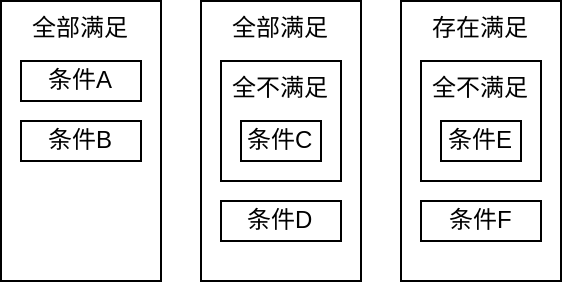
\includegraphics[width=0.8\textwidth]{./imgs/rma-design-adse.png}
	\caption{复合查询条件示例:三个条件分别等价于$ A \land B $,$ \neg C \land D $和$ E \lor F $}
	\label{fig:rma-design-adse}
\end{figure}

零售业务运作的时候,从业者往往需要从数量较为庞大的数据中筛选出所需的一小部分。为了满足这样的需要,管理界面对某些数据类型提供基于布尔代数思想的复合查询条件设计工具。因此从业者并不需要编写布尔代数表达式或SQL \verb|WHERE| 子句就能进行条件复杂查询操作,通过使用鼠标在应用程序提供的用户界面上操作,从业者可以自由组合以下几种类型的条件(\verb|Criterion|):

\begin{itemize}
	\item 字符串字段:前缀为、后缀为、等价于或包含指定字符串
	\item 数值字段:等于、大于、小于指定数值
	\item 日期时间字段:早于、晚于指定日期时间组合
	\item 编号字段:包含于指定正整数集合
	\item 以上条件的集合:其中元素全部符合、任意符合、全不符合、任意不符合
\end{itemize}

输入完成之后,若应用程序没有检测到非法值,将会生成对应的SQL \verb|WHERE| 子句并发送到服务器,服务器将按照对应语句运行SQL查询并返回结果。例如查询名称(\verb|name|)包含“可乐”二字,并且于2025年4月创建(\verb|c_time|)的商品,与以下SQL \verb|WHERE| 子句近似的语句将会被产生:

\begin{verbatim}
	(name like '%可乐%' and c_time > 1743350399 and c_time < 1746028800)
\end{verbatim}

\subsubsection{移动端程序}

\begin{figure}[htbp]
	\centering
	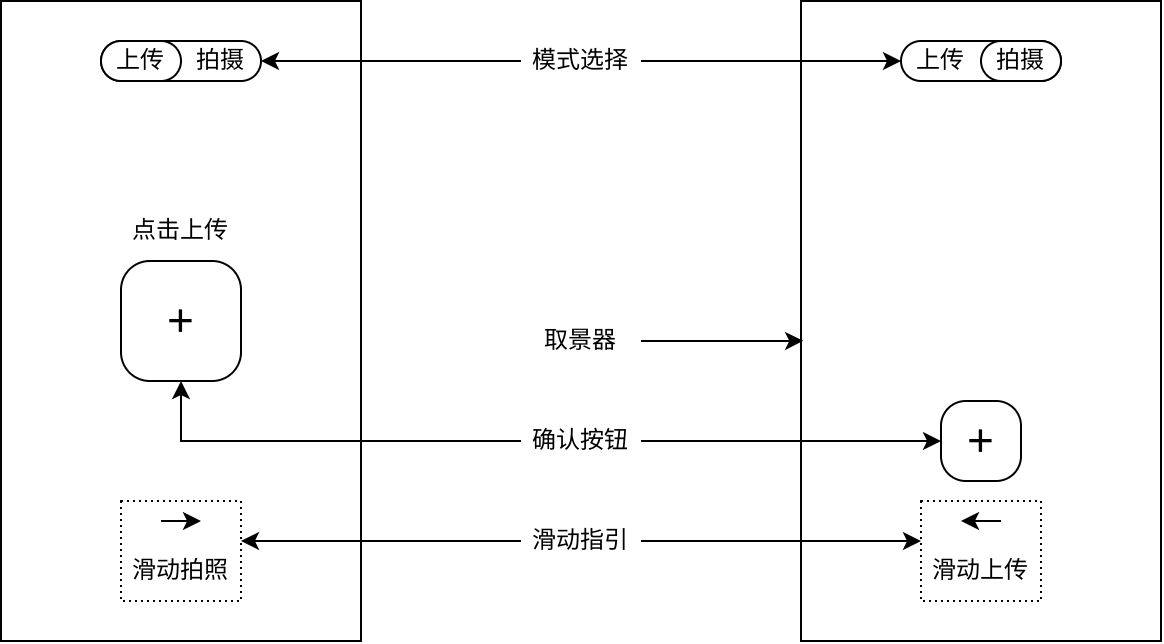
\includegraphics[width=0.8\textwidth]{./imgs/se-picture.png}
	\caption{商家端移动应用程序图像上传部分UI设计}
	\label{fig:se-picture}
\end{figure}

为了进一步降低营业成本,该设计包含一个利用Kotlin语言和Jetpack Compose用户界面库开发的商家端应用程序,用以简化向系统提供图片的流程。从图 \ref{fig:se-picture} 可见,用户可以通过屏幕上侧的标签栏或滑动屏幕空白部分来在上传本地图片和拍摄新照片的界面之间切换。在上传界面上,点击确认按钮可以唤起图片选择界面,用户可以选择一个或多个图片进行上传;在拍摄界面,UI背景部分为取景器画面,在选择完成拍摄角度之后用户只要点击确认按钮即可拍摄照片并即刻上传。

\subsection{结算界面}

该设计具有采用Rust语言和iced实验性用户界面框架构建的用于结算的应用程序。该程序通过与条码识别器、质量传感器和摄像头交互来实现获取商品数据,其后可以在其用户界面上展示待结算的产品。由于具备相应的软硬件支持,该程序可以进行不同计价方式的商品(按件和按质量)的混合结算,一定程度减轻了店员结算的压力和用户自主结算的门槛。

\subsubsection{条码识别器}

为了实现高效识别(计件)商品,结算程序默认通过使用USB HID协议通讯的激光条码识别硬件来读取商品条形码。这种硬件将模拟键盘输入条形码内容,应用程序在商品结算界面将检测是否在较短时间之内从键盘输入符合EAN(European Article Number)-13格式的数据,并在需要时与服务器进行通讯。因为服务器存储条形码的方式是使用字符串而不是数字等其他格式,条形码格式和输入方式方面该设计具有较高的可拓展性,实际部署的情况可以根据不同零售行业细分领域的实际对其进行调整。

\subsubsection{质量传感器}

通过将质量传感器(带有信息传输接口的“电子秤”)整合到结算设备中,设备将具备直接进行计重商品结算的功能,而不需要额外的硬件或设备来进行称重,也不需要额外编写标签并打印。这样,计重商品的结算也可以完全由顾客自助完成,不需要来自店员的帮助。

该设计理论上对质量传感器的规格和信息传输方式没有要求,只要该硬件提供足以断定价格的精度和稳定程度即可使用。本设计默认使用市面上采用率较高的海芯科技HX711电子秤用模数转换器,该芯片成本较为可控,并且在多种平台上具备成熟生态。值得注意的是,HX711的串行通讯功能对相应频率和延迟的要求较为严格。为了解决此问题,本设计包含Arduino UNO 3微控制器开发硬件上采用C++语言和PlatformIO嵌入式开发技术编写的驱动程序,将HX711的专有输出格式转化为了易于处理的文本格式,并通过USB模拟串行接口终端通讯与计算机(和结算程序)相连接和消息传递,以此实现了称重和调零的功能。